\chapter{源代码软件漏洞挖掘基础知识}

为了更好的介绍源代码漏洞挖掘后续章节研究工作,本章首先介绍了源代码的各种中间表示形式;其次,根据所需要的中间表示数量的不同,给予源代码软件漏洞三种描述形式;然后,介绍了程序分析理论基础;最后,介绍了动态符号执行技术。

%常规软件测试方法用于分析源代码软件时尚有诸多问题需要探讨。漏洞挖掘的基本理论方法都源于程序分析与验证领域,尽管很多分析方法都得到了深入的研究,但这些方法通常单独或简单组合后被用于挖掘源代码软件中的漏洞,方法系统性的组合应用尚需要进一步摸索。因此,需要先理清不同分析方法的特点,找准其在系统性漏洞挖掘中的位置,为后续各章做铺垫。
%
%本章主要分析源代码软件测试的基础理论与方法,探讨了典型的静态程序分析、污点分析、符号执行和模糊测试等方法的基本原理及其在漏洞挖掘方面的应用。

\section{源代码中间表示形式}

因为源代码呈现出来的复杂性,在程序分析以及编译器设计技术里,研究人员提出了许多中间表示用于表达程序。其中,语法分析树(Parsing Tree,PT)是语法解析器的直接产出结果,也是生成另外三个基本中间表示即抽象语法树(Abstract Syntax Tree,AST)、控制流图(Control Flow Graph,CFG)以及数据流图(Data Flow Graph,DFG)的基础。

\subsection{语法分析树}

语法分析树能够完全的反映程序语句的结构,以及如何将语句串联成一个完整的程序。输入一个程序,解析器根据语法文件辨别每一个终结符和非终结符,将这些标识符连接之后会得到语法分析树。语法分析树能够展示编程语言元素的类别、结构以及相互之间的关系,表现形式冗余性以及对微小改动非常敏感。图\ref{一个简单的实例程序}是一个简单的示意程序,变量x接收由外部输入函数fun得到的数据,y是x的乘法运算的结果,vul\_fun函数是一个漏洞函数。图\ref{语法分析树示例}是图\ref{一个简单的实例程序}的语法分析树示意图,其根节点是一个函数{(FUNC)},FUNC只有一个复合语句子节点{(CMPD)},复合语句包含两个语句{(STMT)}分别为赋值语句{(ASSIGN)}和跳转语句{(IF)}。


\begin{figure}[h]
\begin{lstlisting}[language=C]
void fun()
{
	int x = input();
	if(x < MAX)
	{
		int y = 2 * x;
		vul_fun(y);
	}
}
\end{lstlisting}
\caption{一个简单的实例程序}
\label{一个简单的实例程序}
\end{figure}


\begin{figure}[htp]
\centering
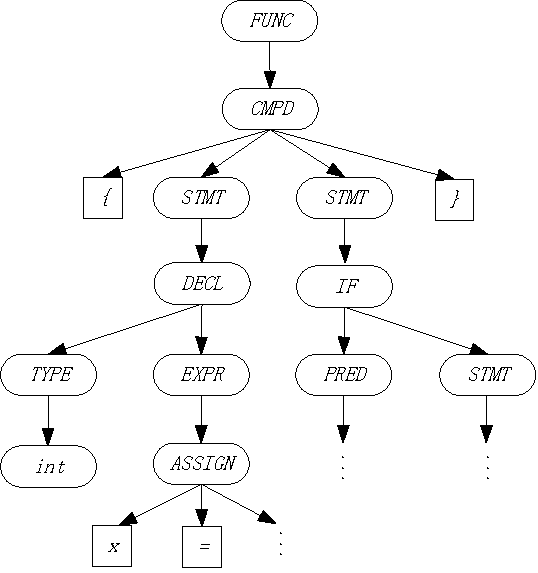
\includegraphics{chap02/语法分析树示意图}
\caption{图\ref{一个简单的实例程序}的语法分析树}
\label{语法分析树示例}
\end{figure}

\subsection{抽象语法树}

抽象语法树是由语法分析树生成的最基本的中间表示,也是生成其他中间表示的基础。抽象语法树详尽的展示了操作数和操作符如何组成程序表达式以及语句,进而展示程序的整体形式。不同于语法分析树,抽象语法树不讲究和程序的每个token表示完全一致,其更偏向于语义的相似性。例如,两个用逗号隔开的变量声明将会产生两个连续的变量声明语法树。

抽象语法树是有顺序的树结构,内部节点是操作符(例如“+”和“=”)而叶子节点是操作数(例如常量和标识符)。图\ref{一个简单的实例程序}的抽象语法树如图\ref{抽象语法树示意图}所示。可以看出抽象语法树中删除了大括号和分号,另外函数调用节点{(CALL)}直接和赋值表达式相连,而语法分析树中在发现函数调用节点之前则需要遍历中间的所有节点。抽象语法树非常适合于简单的代码转换,经常被用来检验源代码的相似性\upcite{baxter_clone_1998,yamaguchi_generalized_2012}。但是抽象语法树不适用于更复杂的代码分析,例如死代码和以及未初始化的变量的检测,其原因是抽象语法树不能提供明显的控制流和数据流信息。


\begin{figure}[htp]
\centering
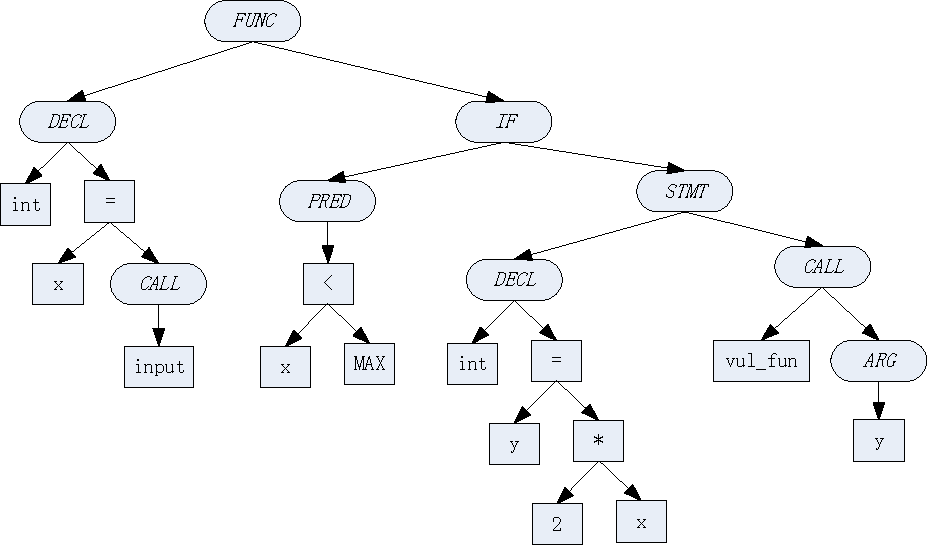
\includegraphics{chap02/抽象语法树示意图}
\caption{图\ref{一个简单的实例程序}的抽象语法树示意图}
\label{抽象语法树示意图}
\end{figure}

\subsection{控制流图}

控制流图能够描述程序语句的执行顺序以及语句之间的支配关系。在控制流图中,一般的顺序语句和控制语句都用节点表示,节点之间用有向边表示控制关系。相对于抽象语法树,控制流图的每条边都有一个标签$true$、$false$以及$\varepsilon$,分别表示控制语句的二类出边以及连接顺序语句的边。图\ref{一个简单的实例程序}的控制流图如图\ref{抽象语法树示意图}所示。

控制流图在程序安全性分析中应用非常广泛,例如辨别已知危险操作的变种\upcite{gascon_structural_2013}、导向符号执行\upcite{sparks_automated_2007}等。另外,控制流图也已经被用在逆向工程中以帮助程序理解。虽然控制流图能够展示语句的执行顺序,但其不能提供数据流信息。在分析可疑漏洞时,不能判定某个语句是否可以被攻击者控制。

\begin{figure}[htp]
\centering
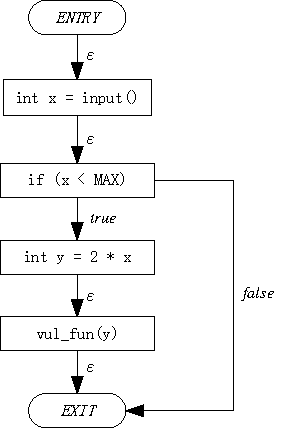
\includegraphics{控制流图}
\caption{图\ref{一个简单的实例程序}的控制流图}
\label{控制流图}
\end{figure}

\subsection{数据流图}

数据流图能够表示语句之间数据依赖关系。在数据流分析中,可以不实际运行程序,直接考察数据的转移情况,从而获取数据流属性信息。图\ref{一个简单的实例程序}的数据流图如图\ref{程序数据流图}所示。变量x从声明语句int\ x=input()传递到两个语句if(x<MAX)和int\ y = 2*x,变量y从声明语句int\ y=2*x传递到vul\_fun(y)。

\begin{figure}[htp]
\centering
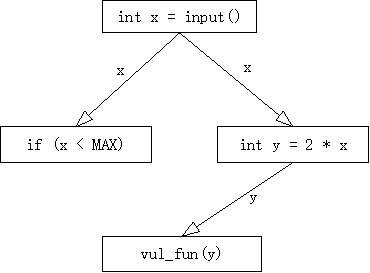
\includegraphics{chap02/程序数据流图}
\caption{图\ref{一个简单的实例程序}的程序数据流图}
\label{程序数据流图}
\end{figure}

\section{源代码漏洞描述}

源代码漏洞挖掘方法通常建立在不同的中间表示之上,根据描述源代码漏洞所需中间表示数量的不同,可以将源代码漏洞描述分为三类\upcite{yamaguchi_modeling_2014}:(1)基于抽象语法树的源代码漏洞描述;(2)基于控制流的源代码漏洞描述;(3)基于污染传播的源代码漏洞描述。不同类别的描述不仅表达的漏洞种类不同,而且对特定漏洞的描述精度也不相同。

\subsection{基于抽象语法树的源代码漏洞描述}

从抽象语法树中可以获取源代码的每一个函数调用、语句甚至每一个操作数和操作符。所以利用抽象语法树可以获取攻击者可控的输入语句,敏感操作语句以及边界检测,但是不能检测出语句之间的关系。通过抽象语法树可以描述以下三类源代码漏洞:

\begin{enumerate}[(1)]
\item 不安全的函数参数使用。不安全的参数是引起源代码漏洞的一个重要原因。例如,格式化字符串漏洞的一个重要特征是传递给$printf$和$sprintf$的格式化字符串能够被攻击者控制。所以若仅仅使用抽象语法树描述时,格式化字符串漏洞可以描述为“$printf$,$sprintf$,$fprintf$的格式化字符串不是常量”;
\item 整数溢出。当内存分配函数(alloc*)的表示内存分配大小的参数存在复杂算术运算时,整数溢出漏洞就有可能发生;
\item 数据类型错误使用。很多漏洞是由于数据类型不正确的转换引起的,例如,造成缓冲区溢出漏洞的一个重要原因就是缓冲区在初始化时,内存大小的运算未进行正确的转换和验证。在进行赋值操作时,如果右操作数的位宽比左操作数大则会发生整数截断。
\end{enumerate}

综上,下面给出基于抽象语法树的源代码漏洞描述。

\begin{definition}
\label{基于抽象语法树的源代码漏洞描述}
基于抽象语法树的源代码漏洞描述可以用一个二元组$(M_0,M_1)$表达,其中,$M_0$和$M_1$表示两个谓词描述。若一个语句节点$v$满足$M_0$而不满足$M_1$,则记$v$为一个满足抽象语法树描述的漏洞。
\end{definition}

利用抽象语法树挖掘源代码漏洞非常有效,但不能完全表达攻击者控制的变量和敏感区域的关系。所以仅仅使用抽象语法树会产生非常多的误报。下一小节将会阐述控制流图是如何帮助部分的解决这个问题。

\subsection{基于控制流的源代码漏洞描述}

因为在控制流图中可以获取程序的执行顺序,很多源代码漏洞需要结合抽象语法树与控制流图才能检测,具体漏洞类型如下所示:

\begin{enumerate}[(1)]
\item 内存泄露。很多漏洞的产生是因为分配的内存没有正确的释放。内存泄露会导致程序崩溃,另外也可以导致其他的漏洞;
\item UAF(Use After Free)漏洞。若一个内存区域在释放后继续使用则会导致程序崩溃或者任意代码执行。此漏洞触发的主要原因是表面上无关的函数调用语句之间复杂的控制流交互关系。使用控制流分析可以轻易的得出内存释放和内存使用之间是否有控制依赖关系;
\end{enumerate}
上面两种情况,产生漏洞的原因都和控制流图上的某一条路径有关。例如,内存泄露是在一条控制流路径上内存被分配给一个变量,但在路径结束之前没有被释放而造成的。下面给出了基于控制流的源代码漏洞描述。

\begin{definition}
基于控制流图的源代码漏洞描述可以用一个四元组\\$(S_{src},S_{end},S_{dst},\{(S^{i}_{cnd},t_i)\}_{i=1...N})$,其中$S_{src}$是一个基于抽象语法树描述的源代码语句,$S_{dst}$是目的语句,$\{(S^{i}_{cnd}),t_i\}$是过程中条件的语法描述和对应的结果,$t_i \in \{true, false\}$。若一个语句节点$v$满足以下三个条件:(1)$v$的语法树子节点中存在$v_{src}$与$S_{src}$相匹配;(2)在$v_{src}$和$v_{end}$之间存在一条控制流路径,且路径中不包含一个节点和$S_{dst}$相匹配,其中$v_{end}$是和$S_{end}$相匹配的语法树节点;(3)对于所有的$1< i \leq N$,若存在一个节点匹配$S^{i}_{end}$,则从此节点的所有出边的标记必须是$t_i$,则记$v$为一个满足控制流图描述的漏洞。
\end{definition}

控制流漏洞挖掘可以通过深度遍历从源节点到结束节点的所有路径,且结束节点不满足目的节点的描述,同时中间节点必须满足相应的条件约束。但是仅仅使用控制流和语法树信息不能跟踪攻击者的信息流,在下一小节中将介绍基于污染传播的源代码漏洞描述。

\subsection{基于污染传播的源代码漏洞描述}

基于污染传播的漏洞描述需要抽象语法树、控制流图以及数据流图三种中间表示形式相结合。符合此标准的源代码漏洞包括:缓冲区溢出、缺乏权限检测以及代码注入等。例如,一类缓冲区溢出漏洞产生的原因是内存拷贝函数中的长度参数没有被有效的验证。检测此类型漏洞就必须首先要获取内存拷贝函数调用的长度参数,然后利用控制流分析判断是否存在条件语句对长度参数做了有效的验证,同时还需要通过数据依赖关系分析判断长度变量是否和输入有数据依赖关系。下面给出了基于污染传播的源代码漏洞的形式化描述。

\begin{definition}
\label{基于污染传播的源代码漏洞描述}
基于污染传播的漏洞可以表示为一个三元组$(S_{src},S_{dst},S^{s}_{san})$,其中,$S_{src}$表示攻击者能够控制的输入语句,$S_{dst}$是导致漏洞的敏感操作,$S^{s}_{san}$是对应的边界检测。对于一个节点$v$,若$v_{source}$是满足$S_{src}$的一个语法树子节点,$v_{sink}$是满足$S_{dst}$的一个语法树子节点,且$v_{source}$和$S_{src}$满足以下个条件:(1)$v_{source}$和$S_{src}$之间存在一条数据依赖路径,即二者有数据依赖关系;(2)对于每一条数据依赖边$e_i = (v_i, v_{i+1})$,存在一条路径$(v_0,...,v_m)$且对于任意$v_k$不满足边界描述$S^{s}_{san}$,$0 \leq k \leq m$,则记$v$为一个满足污染传播描述的漏洞。
\end{definition}

\section{静态程序分析基础}

直观上,静态程序分析是指在不实际运行程序的前提下,对程序进行语义分析。
本节介绍程序的可达状态空间语义和不动点语义,二者是等价的。

\subsection{程序可达状态空间语义}

本节用符号$Var$指代程序变量的集合,符号$Func$指代函数的集合,
符号$Expr(Var, Func)$指代所有基于变量$Var$和函数$Func$构造的表达式,
如赋值表达式$x = y + f(z)$。
给定变量集合$Var$和函数集合$Func$, 用符号$Prog(Var, Func)$指代一段程序源代码。
在计算机中,程序源代码的的一般表示形式为控制流图。

\begin{definition}
给定程序$Prog(Var, Func)$,其控制流图定义为一个三元组$CFG_{Prog} = (L, E, l_0)$,其中,集合$L$表示是程序的所有控制节点,即源代码中程序指令位置;集合$E\subseteq L\times Expr(Var, Func) \times L$
	中的元素连接程序的控制节点,表示程序的控制流;$l_0$表示程序的初始节点。
\end{definition}


直观上,程序的控制流图是一个有向图,图的节点表示指令在源代码中的位置,
图的边表示程序的控制流,同时边上含有一个指令或者一个基本指令块。
一个简单的程序及其控制流图如图\ref{fig-example}所示。
节点$S1$表示程序的初始入口,边$(S1, x=0;n=100, S2)$表示程序文本中顺序执行的赋值指令序列。

\begin{figure}[h]
	\begin{minipage}{.5\textwidth}
		\centering
		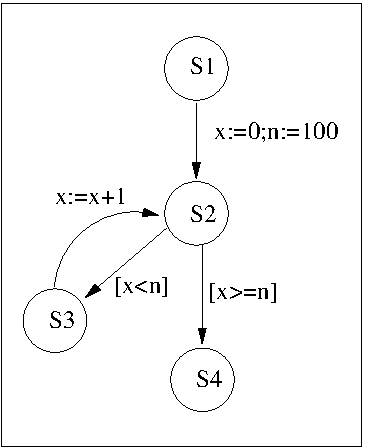
\includegraphics{figures/chap02/example1.pdf}
	\end{minipage}
	%
	\begin{minipage}{.5\textwidth}
		\centering
		\begin{lstlisting}
		int x,n;
		x=0;
		n=100;
		while(x<n)
			x=x+1;
		\end{lstlisting}
	\end{minipage}
	\caption{示例程序及其控制流图}
	\label{fig-example}
\end{figure}


控制流图存在其他的变种,例如编译器LLVM/Clang定义的控制流图将指令放在节点中。
但是,它们所定义的程序语义是等价的。程序的语义通常由状态迁移系统定义。

\begin{definition}
一个状态迁移系统可以定义为一个三元组$T=(S, R, S_0)$,其中,$S$是所有可能状态的集合(也称为状态空间);$R \subseteq S \times S $是迁移关系集合;$S_0$是初始状态集合。
\end{definition}


程序的状态空间由两部分构成:程序指令的位置和程序变量的取值。
给定程序变量集合$Var$,用符号$\textbf{Var}$表示变量所有可能取值集合,
那么,程序的状态空间可以表示为$S = L \times \textbf{Var}$,
其中,$L$是程序控制流图中的控制节点集合。
程序的状态空间可能是有穷集合,也可能是一个无穷集合,
如程序中含有整型变量时,其可能的取值范围为所有整数集合。
同理,程序的初始状态可能有无穷多个,如变量未初始化时。

迁移关系$R$定义了程序的进行一步操作时的状态变化过程,例如,
在图\ref{fig-example}所示程序中,
迁移$((S1, x=*, n=*), (S2, x=0, n=100))$
表示了程序在$S1$位置处执行赋值操作后,变量赋予相应的取值,
其中,符号$*$表示变量的取值为任意值。

一般地,程序的执行可以用一个迁移序列表示,例如,序列
$((S1, x=*, n=*), (S2, x=0, n=100),
(S3, x=0, n=100), (S2, x=1, n=100),
(S3, x=1, n=100) )$表示图\ref{fig-example}
中的程序从初始状态执行,并进入一次循环的状态变化过程。
为表述方便,本节用符号$r\in R$表示一个迁移,序列$r_0 r_1 \cdots r_n$表示一条迁移序列。

一个状态是可达的,当且仅当存在一条执行路径,使得程序能够从初始状态运行到达该状态。
形式化地,状态$s\in S$是可达的,当且仅当存在迁移序列$r_0 r_1 \cdots r_n$,
其中 $r_n = (s_n, s_{n+1})$,使得$s_0$为初始状态,且$s = s_{n+1}$。

给定一些错误状态,或者不安全的状态,
检测程序是否安全的问题可以归结为检测这些错误状态是否可达的问题,
即是否存在一条执行路径,使得程序能够从初始状态执行到某些错误状态。
因此,本质上,程序安全性分析问题可以归结为程序的可达状态空间遍历问题,
即通过遍历程序的所有可能状态空间,检测是否存在不安全的状态。


\subsection{程序不动点语义}

程序的可达状态集合通常是通过计算程序语义泛函的最小不动点得到。
该语义泛函是定义在程序状态迁移系统上的$Post$后继算子。


\begin{definition}
给定状态迁移系统$T=(S,R,S_0)$,
后继算子$Post: S \times R \rightarrow S$
是一个从状态空间和迁移关系到状态空间的映射。
给定状态集合$S_1 \subseteq S$,
$Post(S_1, R) = \{ s\in S | \exists s_1 \in S_1 \wedge (s_1, s)\in R \}$。
\end{definition}

与控制流图类似,后继算子也存在其他变种定义。
在程序分析中,后继算子通常也定义为从状态空间和程序指令到状态空间的映射,
即$Post: S \times Expr(Var, Func) \rightarrow S$。
通过将程序指令进行符号化编码(symbolic encoding),上述两个定义是等价的。
为表述方便,对上述两种定义不做区分。

直观上,给定程序的当前状态和迁移关系,
$Post$算子定义了在下一时刻,程序从当前状态执行一步迁移可能到达的状态集合。

$Post$后继算子作用在状态集合上。
一个状态集合称为程序语义的具体域中的一个元素。
因此,$Post$算子也可以看做是程序语义的具体域上的函数。
给定程序变量集合$Var$,以及变量可能取值集合$\textbf{Var}$,
程序的具体域为幂集$2^{\textbf{Var}}$。
可证后继算子是该具体域上的单调递增函数。

\begin{lemma}
$Post$后继算子是单调递增函数。
\end{lemma}

\begin{proof}
	假设状态集合$S_1 \subseteq S_2 \subseteq S$,
	证明义务为$Post(S_1, R) \subseteq Post(S_2,R)$。
	
	依据$Post$后继算子的定义,
	$Post(S_1, R) = \{ s\in S | \exists s_1 \in S_1 \wedge (s_1, s)\in R \}$,
	那么对任意$s\in Post(S_1, R)$,
	存在$s_1\in S_1$,使得$(s_1, s)\in R$。
	依据假设$S_1 \subseteq S_2$,得知$s_1 \in S_2$,
	故$s\in Post(S_2, R)$。
\end{proof}


一般地,从程序的初始状态,执行$n$次$Post$后继算子,
将得到程序执行$n$步可能到达的状态空间。
理论上,程序的可达状态空间可以通过$Post$后继算子进行数学刻画:
$Reach = \bigcup_{i=0}^{\infty}\{Post^{i}(S_0, R)\}$,
其中,$S_0$是程序的初始状态集合。
程序的可达状态空间可以通过不断迭代运用$Post$后继算子,
直至得到所有可能状态。
然而实际情况下,该迭代计算是不收敛的。
假设上述计算在迭代$n$次后终止,
表示程序的所有可达状态可以在$n$步计算内穷举,
第$n+1$计算不会产生新的状态,即$Post$算子存在不动点。


\begin{lemma}
程序的可达状态空间$Reach$等价于程序语义泛函$Post$算子的最小不动点,
即$Reach = LFP(Post)$。
\end{lemma}

由Knaster-Tarski不动点定理可知,	完备格上的单调函数存在最小不动点。
因此,如果程序语义的对象域构成一个完备格,并且程序的语义泛函是一个单调函数,
那么程序语义的最小不动点一定存在。
然而,即便理论上存在最小不动点,
该迭代过程的计算复杂度也随着程序规模的增长而呈指数级增长。
这就是通常所说的状态空间爆炸问题。

\section{动态符号执行技术}

动态符号执行技术是动态测试用例生成技术的一种,兴起于2005年DART\upcite{godefroid_dart:_2005},又被成为白盒Fuzzing。有别于静态分析,动态符号执行技术通过程序插桩,在程序运行时收集分支语句上的与输入相关的谓词表达式,然后调用约束求解器生成测试用例以趋使下一次执行到不同的路径。近年来动态符号执行技术在软件测试研究领域越流行开来,主要有两个原因:(1)程序运行产生足够的运行时信息使得测试不会产生大量的误报;(2)每一测试用例都会产生新的路径,使得动态符号执行在提高代码覆盖率上非常有效。


%该技术以
%一组随机生成的数据作为输入,通过分析程序动态执行信息来获取可达路径对输
%入数据的约束,并在遇到受输入数据控制的分支跳转时将收集到的约束,输出至
%可满足模求解器(SMT Solver),用以判定另一分支路径是否可达。若可达,求解
%器则给出覆盖目标分支路径的测试用例,并利用生成的测试用例发掘目标分支路
%径中的软件缺陷。典型系统包括微软研究院的 DART\upcite{godefroid_dart:_2005}、 SAGE\upcite{godefroid_sage:_2012}、SmartFuzz\upcite{molnar_dynamic_2009}、 Hunter\upcite{hunter__2010}等。

%作为动态测试用例生成技术的前身,传统的符号执行技术使用符号变量代替
%待测程序单元的实际输入值,之后使用替代的程序执行语义模拟执行待测程序单
%元。在执行过程中遇到的包含符号变量的条件表达式即为可决定程序执行路径的
%路径约束。待测单元的所有路径可通过对路径约束的真值赋值表示为一棵二叉执
%行树,其中每一个内部节点代表了一个分支路径选择。通过在树上深度优先的回
%溯搜索,寻找、判定预期路径约束的可达性并寻找对应的数据样本,满足预期执
%行路径的实际输入值即可被产生。但是,这种传统方法在处理大规模的或者较为
%复杂的待测单元时存在问题。例如,如果某一个路径约束的可满足性是无法判定
%的,那么传统的符号执行技术就无法继续进行搜索,从而导致了不佳的覆盖率;
%对于包含复杂数据类型(例如指针、数组)的程序,依靠静态的模拟执行无法精
%确的求解路径约束,同样也会在真实测试中导致低覆盖率。
%
%动态测试用例生成技术的提出正是为了解决传统方法的不足,其基本想法在
%于将传统符号执行中的符号输入与具体值输入相结合。动态符号执行采用实际输
%入值真实地执行待测程序单元,在程序执行的过程中进行符号执行过程构建路径
%约束,同时记录通过符号变量表达的抽象程序状态,以及用实际数值表达的真实
%程序状态。由于待测程序被真实的执行了,所以所收集到的路径约束是遵循程序
%本身的语义的,且是精确的。因而在动态方法中不会出现如静态方法的虚假警报,
%并且也有助于对复杂数据结构进行分析处理。另外,由于程序的真实状态被记录,
%一旦遇到不可判定的路径约束,可使用变量的实际值替代符号值,使后续的路径
%探索过程可以继续进行。因为相比传统方法,可达到更高的覆盖率,所以其被广
%泛的应用在了程序测试与验证中,并且有相当多的工作扩展了动态符号执行的适
%用范围,如通过引入额外的内存模型以更精确的处理数组;通过引入额外的分析
%方法提高对循环的覆盖率等。

%动态测试用例生成技术主要目标有两点:(1)为待测程序单元自动的生成可
%达到较高覆盖率的测试数据;(2)在动态过程中寻找待测程序的缺陷。
动态符号执行技术的一般流程如图\ref{动态符号执行流程}所示。 其处理流程如下:
\begin{enumerate}[(1)]
\item 以某一具体输入启动目标程序,该输入可随机生成;
\item 在目标程序的地址空间中,将输入对应的内存位置标记为符号变量;
\item 对目标程序的每条指令,将其语义计算转换到基于符号变量的符号表达式
域下,计算其抽象语义,更新对应的符号变量状态。对于符号计算相关的流程转
移类的指令,计算其对应于当前具体执行路径的分支谓词,并累积至当前路径对应
的全局约束条件;同时计算另外一条分支对应的符号约束,通过约束求解进行可
满足性判断,确定该路径的可行性。在可行的情况下,将分支对应的路径约束保
存入调度队列;
\item 若调度队列非空,则从调度队列中抽取出一个分支约束,计算出满足约束
条件的输入的具体值,回到步骤(1)对该路径进行符号分析;否则,即结束对目
标程序的符号分析。
\end{enumerate}

\begin{figure}[h]
\begin{center}
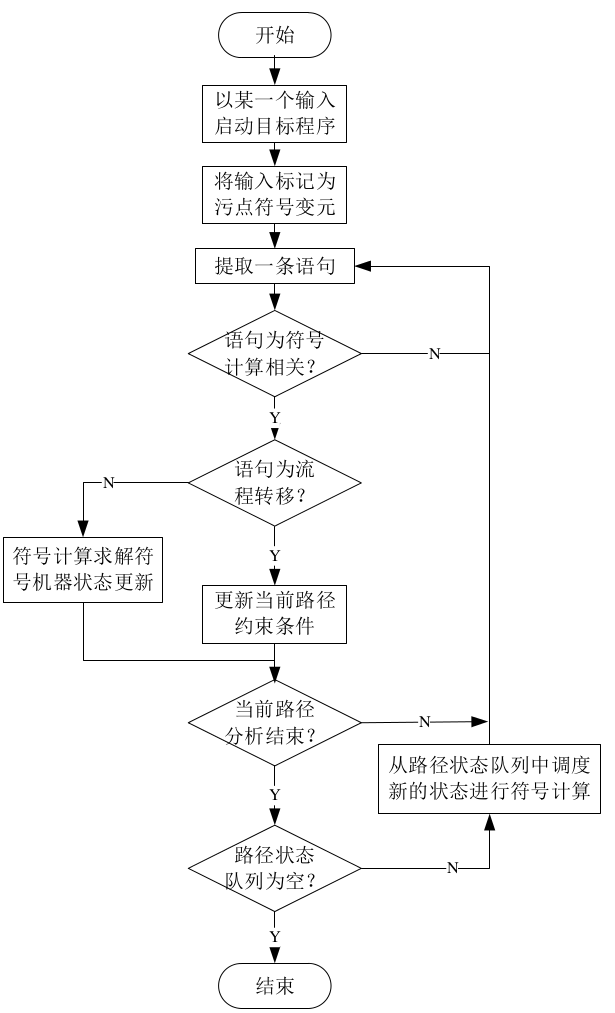
\includegraphics[scale=0.4]{chap02/动态符号执行流程}
\end{center}
\caption{动态符号执行流程}
\label{动态符号执行流程}
\end{figure}

论文第五章使用的符号执行工具是KLEE\upcite{cadar_klee:_2008}。KLEE是由Cadar与2008年开发的动态符号执行工具。KLEE依托于LLVM编译器,支持的最高的LLVM版本是3.4。KLEE执行LLVM字节码,记录程序中不同的路径,使用运行时检查器(Runtime Checker)检测程序错误,并利用约束求解器求解路径约束产生测试用例。KLEE能够获取很高的代码覆盖率并且发现深层次漏洞。

KLEE的架构如图\ref{KLEE架构}所示。和很多其他的符号执行工具一样,KLEE包含的一个主要的组件是metaSMT接口,支持多种约束求解器,例如Z3,STP,Boolector。KLEE还包含多种搜索策略即深度优先、宽度优先、随机搜索、最大覆代码覆盖率以及混合搜索策略,且提供了基本的搜索策略接口,可以方便的自定义搜索接口。此外,KLEE还实现了环境交互模型,即利用自己编写的数据读写函数代替程序原始调用的函数,例如open,read等。此做法有三个好处:(1)简化版的函数能够减轻原始复杂程序造成的路径爆炸;(2)能够根据代码规范模拟闭源的代码库,使得符号执行能够顺利执行;(3)通过模拟网络通信可以符号执行网络程序。尽管环境建模有这些优点,但是程序的模拟代码都是使用者手动编写的,每次遇到不同的程序需要重新编写。

\begin{figure}[h]
\begin{center}
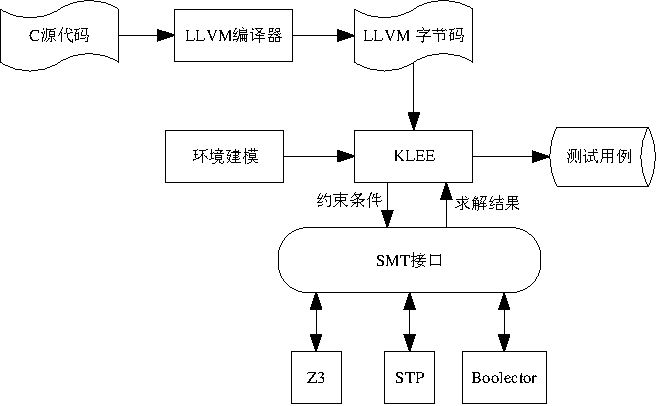
\includegraphics[scale=1.2]{chap02/KLEE架构}
\end{center}
\caption{KLEE架构}
\label{KLEE架构}
\end{figure}


%抄wb
%\section{模糊测试}
%模糊测试是指通过不断给目标软件发送各种畸形数据来挖掘其中可能隐含的
%安全漏洞,是一种强制性的漏洞挖掘方法。模糊测试与传统白盒方法不同,不需
%要分析程序源代码;也与传统黑盒测试只关注用例输出是否与预期相符有所不同,
%模糊测试只关注目标软件是否出现了异常\upcite{sutton_fuzzing:_2007}。
%
%\subsection{模糊测试的一般过程}
%具体模糊测试方法根据目标软件、输入格式、运行平台等不同的测试需求各
%不相同,但基本过程是一致的,包括以下几个步骤:
%
%(1)确定输入向量
%
%由于可利用漏洞都是由于软件在处理用户输入时没有经过正确的校验。因此,
%输入向量的枚举是模糊测试方法取得成功的关键因素。所有软件能够接收的数据
%都应该被认为是输入向量的组成部分,主要包括文件输入、网络数据包等。
%
%(2)生成测试用例
%
%在了解输入特性后,就可以根据变异或随机构造的方式生成测试用例。根据
%目标软件及其数据格式的不同,用例的生成方式也各不相同,可以采用随机生成
%的方式,也可以采用基于正常样本变异的方式,或者采用启发式规则生成的方式
%等\upcite{robertson_run-time_2003} 。一般模糊测试系统会生成海量测试用例,而其中大部分的用例都是无效
%的。因此,一般需要深入分析目标软件,构造更加有效的用例。
%
%(3)执行测试用例
%
%这一步通常与用例生成并行进行,执行过程一般包括启动目标软件、适用测
%试用例激励目标软件等。
%
%(4)异常检测与分析
%
%尽可能多地触发软件异常是模糊测试的目标。因此在测试目标软件时,应实
%时监测一切可能的异常、崩溃等信息,在异常发生时记录和保存重要的运行状态
%信息。并进一步分析软件异常的可利用性,合并重复的异常信息等。
%
%\subsection{测试用例生成方法}
%
%模糊测试是一种试图遍历软件输入空间的方法。因此,测试用例生成方法的
%好坏是影响模糊测试有效性的重要因素。测试用例生成方法大体上可分为两大类:
%基于变异的方法和基于生成的方法。
%
%(1)基于变异的方法
%
%这种方法从一个有效的输入样本开始,随机地变异样本中的部分数据来生成
%新用例。这是一个比较原始的方法,几乎不需要被测软件的任何先验知识,实现
%起来非常简单且通用性强。但这种方法效率很低,因为被测软件浪费了大多数的
%时间处理无效的输入数据。因此,后续有很多改进的方法,比如基于静态分析辅
%助的方法\upcite{wu_new_2009,lanzi_smart_2007,rawat_offset-aware_2011},基于运行时反馈方法 \upcite{ganesh_taint-based_2009,bekrar_finding_2011},基于遗传算法的方法\upcite{rawat_evolutionary_2010,liu_vulnerability_2008,cordon_ten_2004} 等。
%
%(2)基于生成的方法
%
%随机生成是最简单的生成策略,该方式只是简单地产生大量伪随机数据用于
%激励目标软件,能否触发异常有很大的概率性。因此,此法虽然简单却并不常用。预生成测试用例也是一种常见的生成策略,该方式首先研究目标软件的输入
%规范说明,以了解其支持的输入数据结构和取值范围,然后生成硬编码的畸形数
%据以测试边界条件或违反规约\upcite{liubiao__2014} 。这种方式生成的用例针对性强,因此测试效
%率相对较高。但是,创建这些用例需要事先完成大量的分析工作,自动化程度不
%高,而且有的输入规范并不可得。还有一种就是基于符号执行的生成方法,如
%SmartFuzz\upcite{molnar_dynamic_2009} 、SAGE\upcite{godefroid_sage:_2012} 等,这些系统将正常测试数据当作符号值,收集目标软件
%处理正常输入时的路径约束,通过约束求解生成新用例。理论上符号执行的方式
%能够生成精准的用例,但实际测试过程中由于面临路径爆炸、分析精度受限、指
%针分析难等问题,其应用场景也受到限制。
%
%\subsection{模糊测试框架}
%
%模糊测试框架是模糊测试过程的通用化实现。通过使用测试框架可以简化被
%测软件输入的表达、被测目标的监测和异常分析管理等,能够极大地提高模糊测
%试的自动化水平。虽然已经存在很多模糊测试框架,比如antiparser\upcite{noauthor_antiparser_nodate} 、
%Peach\upcite{noauthor_peach_nodate} 、Sulley\upcite{noauthor_sulley:_2017}、AUTODAFE\upcite{noauthor_autodafe_nodate} 等,但它们并不提供通用的解决方案,有其
%特定的适用范围。一般来讲,使用模糊测试框架可以实现功能复用,便于经验的
%积累和分享;但同时也必须花大量时间来学习框架,某些测试功能还可能因为框
%架的限制而无法实现。
%虽然模糊测试缺乏形式化模型和理论基础,然而模糊测试却是迄今为止发现
%未公开漏洞数量最多的挖掘方法。模糊测试实际上利用了漏洞挖掘问题的可猜解
%性和可验证性,虽然无法准确回答是否能检测到漏洞、是否能检测出所有漏洞等
%问题,却能够挖掘出很多意想不到的漏洞。因此,在其他挖掘方法效果不理想时,
%模糊测试可以作为一种很好的补充手段。论文在分析可编程类软件时,就采用了
%模糊测试的思想,基于模糊编程的思路对被分析软件进行测试。
%%抄wb

%\section{基于机器学习的漏洞检测方法}



\section{本章小结}

本章介绍了源代码漏洞挖掘中所使用的四种中间表示:语法分析树、抽象语法树、控制流图以及数据流图。在分析了各类中间表示表达能力的基础上,根据需要的中间表示数量的不同,将源代码软件漏洞描述分为三类,即基于抽象语法树的源代码漏洞描述、基于控制流的源代码漏洞描述以及基于污染传播的源代码漏洞描述。最后,介绍了第五章所使用的静态程序分析基础以及动态符号执行技术。
